\chapter{Capturing and Recording Media}%
\label{cha:capturing_recording_media}

\begin{figure}[htpb]
    \centering
    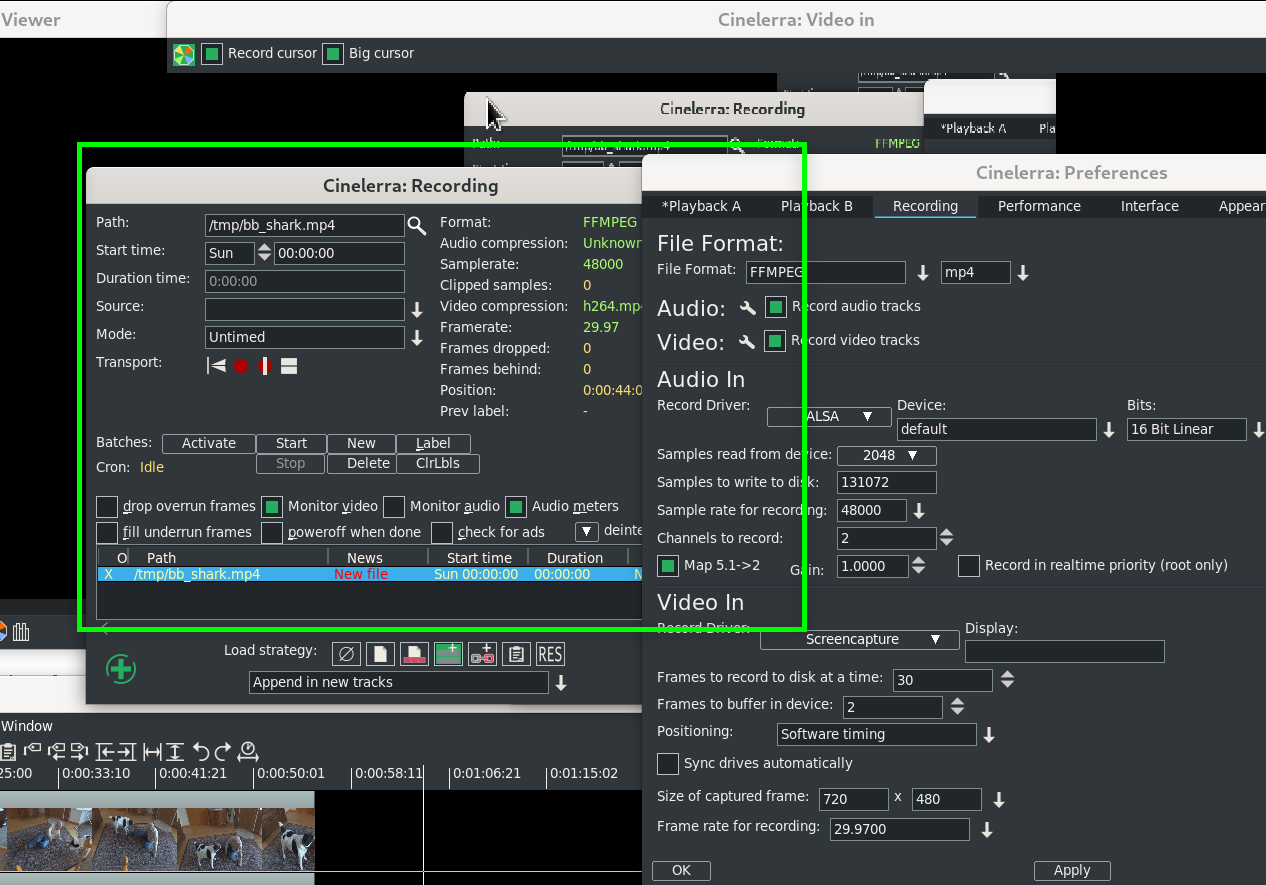
\includegraphics[width=\linewidth,keepaspectratio]{recording07.png}
    \caption{Actual Recording Session - note the bright green boundary box and the big arrow cursor
within the "Video In" window}
    \label{fig:recording07}
\end{figure}

This section covers the areas of capturing media from the web or television by the use of recording.

Access the Record function via \texttt{File} $\rightarrow$ \texttt{Record}\dots The recording application really only does one thing, capture media from some external source and write it onto a file in a specified way.

\vspace{2ex}
\begin{tabular}{lll}
    Path: & output media file path & \\
    
    Start time: & weekday/time of day & to begin capture\\
    
    Duration: & hrs:mins:secs & until end of capture\\
    
    Source: & channel/device input & selection of input subsource\\
    
    \multirow{2}*{Mode:} & timed & use start time/duration \\
    
    & untimed & use transport controls\\       
\end{tabular}

\vspace{2ex}
The media file will be written using the format and codec specified in the \texttt{Settings $\rightarrow$ Preferences $\rightarrow$  Recording tab}, which you will need to set up first.  See the \hyperref[sec:recording]{Settings/Preferences} section for parameters. Only ffmpeg can record both audio and video simultaneously, and some ffmpeg formats require too much cpu to do a realtime compression.  A setting which is more likely to be usable (requires less cpu/memory for realtime encoding) is \texttt{ffmpeg $\rightarrow$ qt $\rightarrow$ mp4.qt} with bitrates like $audio/256000$ \& $video/6000000$.

\section{Record Web Media in real-time}%
\label{sec:record_web_media_rt}

Below describes the necessary steps for recording freely available media from the internet for your own personal use.  You have to be on a system using pulseaudio, such as ubuntu, fedora, centos.

\begin{enumerate}
    \item Start \CGG{} and select \texttt{Settings $\rightarrow$ Preferences $\rightarrow$  Recording} From a terminal (with a wide text window) run: \texttt{pactl list}. You will see all of the audio sources and sinks on your system. Identify the source associated with the normal output your system uses. Example: \textit{Source $\#1$}. Locate the source which monitors your normal audio output.  For example: \textit{front stereo}.        
    \item Choose a File Format and File Type (for example: FFMPEG \& qt).
    \begin{itemize}
        \item Check \textit{Record audio tracks}.
        Click \texttt{Audio wrench} tool:
        \begin{itemize}
            \item Select \textit{mp4}, for example.
            \item Set \textit{Bitrate} ($256000$ is a reasonable number).
        \end{itemize}
        \item Check \textit{Record video tracks}.
        \item Click \textit{Video wrench} tool:
        \begin{itemize}
            \item Select \textit{mp4} video, for example.
            \item Set \texttt{Bitrate} $1000000 - 4000000$ (bigger=better, but more cpu)
        \end{itemize}
        \item Select \texttt{Audio In $\rightarrow$ Record Driver:  ALSA} (or whatever you have instead)
        \begin{itemize}
            \item Set the \textit{Bits}: \textit{16 Bit Linear} (probably, because reasonable and fast)
            \item Select \textit{Device}: the source from above \textit{pactl} list search, for example Source $\#1$
            \item Samples read from device: aprox dev buffer size ($2k-16k$ probably)
            \item Samples to write to disk: $131072$ (a good size)
            \item Sample rate for recording: $44100$ (will automatically change)
            \item Channels to record $2$ (probably)
            \item Uncheck Map $5.1 \rightarrow 2$
            \item Gain $1.0$
        \end{itemize}
        \item Select \texttt{Video In $\rightarrow$ Record Driver}:  \texttt{Screencapture}
        \begin{itemize}
            \item Set the \textit{Display}: leave blank (probably) or use "$:0.0$" (default screen/display)
            \item Frames to record to disk at a time: $30$ (a good number)
            \item Frames to buffer in device: $(2-6)$ (probably)
            \item Positioning: \texttt{Software Timing} (important)
            \item Uncheck: \texttt{Sync drives automatically}
            \item Size of captured frame: $720x480$ (this is your choice, actual capture size; $600x320$ youtube)
            \begin{itemize}
                \item This defines a \textit{screen capture} rectangular area on the display.
                \item Try to make it the size you need to cover the screen playback area.
            \end{itemize}       
        \end{itemize}
        \item Frame rate for recording $23.97 fps$ (a good choice, not all choices work)
        \item OK
    \end{itemize}
    
\end{enumerate}

When recording from the screen, a large green-colored boundary box appears to allow you to easily frame the screen area to be recorded when you move it around to where you want to position it.  In addition there are \textit{record cursor} and \textit{big cursor} check boxes which allow for also recording the cursor and for making the cursor bigger. 
You can see the bright green boundary box and these checkboxes around the middle at the top in
figure~\ref{fig:recording07}.

Screenshot to illustrate some appropriate settings which are described above/below the image (figure~\ref{fig:recording01}).

\begin{figure}[htpb]
    \centering
    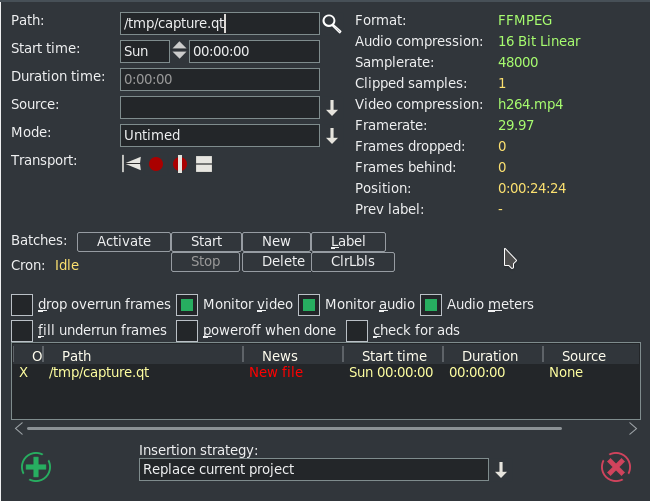
\includegraphics[width=0.8\linewidth]{recording01.png}
    \caption{Recording window with typical settings}
    \label{fig:recording01}
\end{figure}

\begin{enumerate}[start=3]    
    \item Make sure the Compositor window is up since you will want to see the captured media later. From the main window press (lower case "r") (move windows and resize if needed) Using the mouse pointer, mouse over the \textit{Video In} Recording monitor display. Press and hold the left mouse button and drag the display until the desired target screen capture area is properly positioned inside the record monitor \textit{Video In} display.  At first this may seem confusing, but keep in mind that what you are actually doing is positioning the portion of your monitor display you want to capture over the \textit{Video In} window.
    \item From the \textit{Recording window} select a Path file name for the recording.
    \item Select mode untimed.
    \item Make sure the \textit{monitor audio} is unchecked else audio becomes looped and is very loud.
    \item Press Transport \textit{start recording} (red circle button).
    \item Operate the playback of the media source, i.e. start playing the web video.
    \item When the media ends, stop on the playback application.
    \item Press Transport \textit{stop recording} button (white square button).
    \item Before clicking chk-Ok, be sure to set the \textit{Insertion Strategy}.
    \item Press chk-Ok to review the capture, or "X" to cancel/dismiss application.    
\end{enumerate}

Two things are happening during recording, the data is being written, and it is being rendered.  When recording, if video and audio are not in sync, it will usually be video behind audio as opposed to the other way around because video is more difficult to decode.  During recording, video frame and audio sample positions are checked and efforts to maintain synchronization are used.   Below is an explanation for some of the less obvious settings for recording as shown in the previous screenshot.
\paragraph{Frames dropped} more input than cpu(s) can process.  This is the number of frames dropped when the system is too slow to keep up with the video.  This value serves as a warning that it is behind and is dropping frames to keep up.  You might want to consider stopping to make some parameter adjustments and start over to reduce drops.
\paragraph{Frames behind} active input buffers.  This is the number of frames that the video is behind and it will drop frames to get caught up.  \textit{Frames behind} depends on the synchronization source, for example, time as the synchronization.  This means that frames are not being written as fast as they are being captured and can occur when the system is too slow to keep up.  This situation can happen with older systems or cpus where there is more input then can be processed in a timely manner.  So that when there are \textit{Frames behind}, frames will be dropped.

The algorithm for determining how many frames to drop is as follows:

\begin{itemize}
    \item If the number of frames behind $> 3$, only $3$ frames will be dropped before it will then do $1$ frame;
    \item if the number of frames behind is $2$, only drop $1$ frame;
    \item if only $1$ frame behind, no frames will be dropped.
\end{itemize}
\paragraph{Drop overrun frames} checkbox when enabled, frames will be dropped.  Drops occur when you capture a frame and there is no storage space available to save it, usually because buffer space is exhausted.  This situation can occur when there are too many frames coming in too fast and the I/O system is not keeping up in emptying the buffers.
\paragraph{Fill underrun frames} checkbox if enabled, duplicate last frame when no input frame ready for output.  As the tooltip states \textit{write extra frames when behind}. This is desirable in order to keep audio and video synched with regards to sample and frame rates.  Use underrun padding to fill frames when the input capture rate is lower than the output frame rate.  Since demand is constant, you have to output something, so the last frame is duplicated as many times as needed to keep up.  You should stop and adjust the frame/sample rates to match the input if not filling underruns, then start over.  This situation can occur if the input stops for some reason like lightning interrupts the signal or the internet connection is too slow.
\paragraph{Transport controls} these control buttons mimic the functions of tape recorders from the old days.

\begin{itemize}
    \item \textit{Reverse button/left arrow} --remnant from the past; does the same as the Start button really.
    \item \textit{Red round button} --this is the Start button to start recording.
    \item \textit{White square} --this is the Stop button to stop recording.
    \item \textit{Red round button with white line} --start recording in single frame mode.  The way this works is to just \textit{take a picture now, take a picture now\dots}  The reason to use this mode is to get a still shot like you would with a camera.  Sometimes input is continuous, for example looking at stars with a telescope -- surveillance goes on for hours, but you just want to take a picture now when something of significance interest comes up
\end{itemize}
\paragraph{Cron} The batch recording watcher, cron, is either \textit{Idle} or \textit{Active}.  When you start or stop batch recording at specific times, there is a cron thread watching timers to perform the timed action.  Idle/Active indicates whether the timers are running.
\paragraph{Position} this is a timebase which tracks frames/samples when obeying frame/sample rate.  When a recording starts, it resets to 0.  Timing is against audio (when available).  Audio time and video time are based on position.
You can select synchronization time source \textit{Positioning} in:

\texttt{Settings $\rightarrow$ Preferences} under the \textit{Recording} tab.

\noindent Possible choices for time base are:

\begin{itemize}
    \item \textit{Presentation Timestamps} --use time code which is in both the audio and video media input stream. Uses these timestamps to sync the 2 streams.
    \item \textit{Device Position} --this is the device hardware position of where you are.  It is usually only on the audio side.
    \item \textit{Sample Position} --Sample $\#$ or frame $\#$ divided by frame rate tells you where you are.
    \item \textit{Software Timing} --usually used for things like YouTube; it just will \textit{take a picture now} \dots \textit{take a picture now} \dots over and over again until you tell it to stop.    
\end{itemize}

Positioning \& Timing needs more detailed explanation for complete understanding and application.  The overall goal is to maintain media stream timeline synchronization.  The reason for providing different \textit{Positioning} options is that different input media may have different timebase standards.  Additionally, the input may be damaged.  Damaged data can skew the timeline during presentation.  The timebase standards make it possible to correctly resynchronize the media presentation to the original time position.  For example, the transport layer may have timestamps provided in it.  These timestamps record \textit{audio time} and  \textit{video time} and are called \textit{presentation timestamps}.

The kind of positioning used depends on the input device and the media format.  In the transport stream example, the media has already been coded at least once as a stream and contains position information.  In other situations, sample position or device position can provide timeline position.  If the input device provides data at a variable or asynchronous rate, then software timers can provide timeline position.  Sample position is position from the perspective of software, and device position is position from the perspective of hardware.  The difference is buffer time.  Device position is usually more accurate, but may not be available, or may contain errors.

Examples of media which usually has a particular type of positioning is:

\begin{enumerate}
    \item mpeg has timestamps therefore Presentation Timestamps is a good recording choice;
    \item raw media streams/screen capture have no timestamps, so tell it time via Software;
    \item a web cam may supply data at variable rates, so again you would use \textit{Software timing};
    \item an example of Device Position is audio (timestamps can come off the device);
    \item if Software Positioning working for you, try Sample Position for really bad audio.
\end{enumerate}

Other \textit{Recording} settings are more pertinent to capturing and editing broadcast television with all of its many commercials.  Their usage will be explained in more detail in a later section.
\paragraph{Label} create a label.  During capture, put a time marker at the designated spot.  When the recording 
gets pulled in later for review, you will see a green arrow marking the spot that was clicked.
\paragraph{ClrLbls} clears all of the previously set labels.
\paragraph{Check for ads} check for commercials.  In real time, labels are added when a commercial that matches
a previous ad is already in the database (the TDB, Traveling Data Base).

One other noted new feature is a new choice for recording -  \texttt{V4L2 MPEG}.  Some digital tuners now stream mpeg data for broadcast data streams.  V4l2 has been upgraded to be able to process data from these device streams.  Figure~\ref{fig:recording02} shows the available options to include v4l2 mpeg.

\begin{figure}[htpb]
    \centering
    \includegraphics[width=0.8\linewidth]{recording02.png}
    \caption{new feature V4L2 mpeg}
    \label{fig:recording02}
\end{figure}

\section{Digital Video Broadcasting (DVB)}%
\label{sec:digital_video_broadcasting}

You can do real-time capture of a full transport stream of Broadcast TV.  Record television programs using \CGG{} by setting up ahead of time to start recording later at the specified time.  Then you can use \CGG{} to watch later and easily fast forward through the commercials or edit the program, deleting the commercials, to watch uninterrupted.  Some details may be slightly different than what it is in the United States.  There are 3 requirements you must have to take advantage of this capability.

\begin{enumerate}
    \item You need to have a suitable DVB Adapter such as the Hauppauge WinTV-HVR 950Q usb adapter. Make sure it is the linux version, not the new version.
    \item Your DVB adapter on your PC should connect to a broadcast antenna input.
    \item For now, you may have to run as the \textit{root} user.
\end{enumerate}

\subsection{Overview}%
\label{sub:overview}

There is a lot of detailed explanation below to be thorough, but an overview is presented here.

\begin{enumerate}
    \item Set up Record Preferences.
    \item Scan the Channels.
    \item Watch TV by selecting the desired channel.
    \item Or set up a batch job to record a program and watch later via Ctrl-Alt-s in the main window.
    \item Or record a currently running program by using the buttons in the Record window.
    \item Load a previously recorded program.
\end{enumerate}

\subsection{Initial Setup for DVB Capture}%
\label{sub:initial_setup_dvb_capture}

Listed below are the steps for the initial DVB setup.  Setup will be preserved until you make changes.

\begin{enumerate}
    \item Start \CGG{}, and click \textit{Settings $\rightarrow$ Preferences $\rightarrow$ Recording}
    \item Select \textit{File Format} checkbox: \texttt{Realtime TOC} (Table of Contents)
    \begin{itemize}
        \item It is not necessary to set File Format at this point as it will automatically be set later.
        \item Check \textit{Record Audio Tracks}.
        \item Check \textit{Record Video Tracks}.
    \end{itemize}
    \item Select \texttt{Audio In $\rightarrow$ Record Driver: DVB}
    \begin{itemize}
        \item Set the \texttt{adapter path = /dev/dvb/adapter0} (probably)
        \item Set the \textit{adapter dev = 0} (probably)
        \item Set the \textit{Bits: 16 Bit Linear} (probably)
        \item Check: \textit{Follow audio config}
        \item \textit{Samples read from device}: $2048$ or approximate dev buffer size ($2k-16k$ probably)
        \item \textit{Samples to write to disk}: $131072$ (a good size)
        \item \textit{Channels to record}: 2
        \item Uncheck \textit{Map} $5.1 \rightarrow 2$
        \item \textit{Gain}: $1.0$
        \item Uncheck: \textit{Record in real-time priority}
    \end{itemize}
    \item Select in \textit{Video In}: \qquad \textit{Record Driver: DVB} (note: File Format above changes to \textit{MPEG Stream})
    \begin{itemize}
        \item Set the \texttt{DVB adapter} path = \texttt{/dev/dvb/adapter0} (probably)
        \item Set the adapter \textit{dev} = 0 (probably)
        \item Check: \textit{Follow video config}
        \item \textit{Frames to record to disk at a time}: 30 (a good number)
        \item \textit{Frames to buffer in device}: 2 ($2-6$ probably)
        \item \textit{Positioning: Presentation Timestamps} (\textbf{this is important and may not be already set})
        \item Uncheck: \textit{Sync drives automatically}
        \item \textit{Size of captured frame}: $720x480$ (will automatically change)
        \item \textit{Framerate for recording}: $29.97$ (will automatically change)
        \item Click OK
    \end{itemize}
\end{enumerate}

Figure~\ref{fig:recording03} shows the Preferences window as a good example of what you should see.

\begin{figure}[htpb]
    \centering
    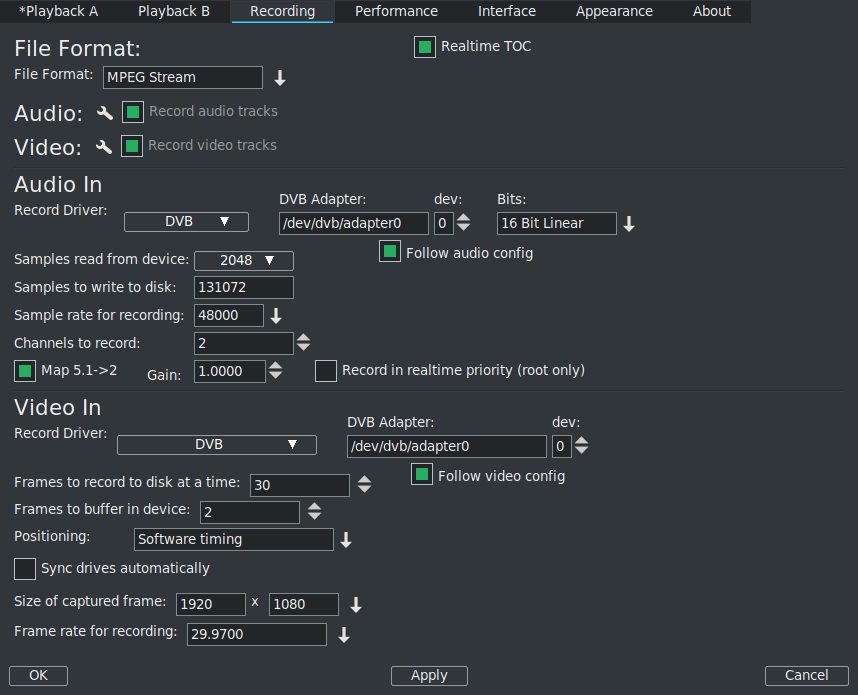
\includegraphics[width=0.99\linewidth]{recording03.png}
    \caption{Example of the Recording settings}
    \label{fig:recording03}
\end{figure}

Scan the channels once the devices are setup by performing the following.

From the main window pulldown use:  \texttt{File $\rightarrow$ Record}  (lower case \textbf{r}) \& \textit{resize windows}.

\begin{itemize}
    \item Two windows appear --  the \textit{Recording} and the \textit{Video In}.  The Recording window should have \texttt{Monitor video} checked and \textit{Monitor audio} unchecked.  Remember to check the Monitor audio later when you want to listen to a TV program.
    \item On the \textit{Video In} toolbar, click the \textit{antenna} button (\textit{Edit channels} tool tip).
    \item When the \textit{Channels} window opens, click \textit{scan} -- \textit{Scan confirm} window appears.
    \item Make sure \textit{Freq table NTSC\_DVB}, \textit{Norm NTSC}, and \textit{input0} are chosen automatically.
    \item Click OK and then wait for scan to end which may take several minutes.
\end{itemize}

Figure~\ref{fig:channels01} on the left shows the Channels window and the popup waiting for scan confirmation.  On the right side is the usual Recording window with the Video in window hidden behind.

\begin{figure}[htpb]
    \centering
    \includegraphics[width=0.99\linewidth]{channels01.png}
    \caption{Clockwise: Channels window; Video In (behind); Recording and Scan confirm}
    \label{fig:channels01}
\end{figure}

Figure~\ref{fig:channels02} shows scanning in progress.  Note the \textit{Video In} with the antenna icon (3rd symbol).

\begin{figure}[htpb]
    \centering
    \includegraphics[width=0.99\linewidth]{channels02.png}
    \caption{Scanning in progress ($6\%$)}
    \label{fig:channels02}
\end{figure}

Any time after the channels have been scanned, you can edit them from the \textit{Recording} window channel selection dialog (shown on left of screenshot above, such as \textit{Sort}).  You do not have to scan the channels every time as they are saved in a database referred to as the \textit{channel-db}.

\begin{itemize}
    \item Click chk-OK when done scanning channels and making any edits you want.
\end{itemize}

\noindent After the channel-db is ready, you can watch any of the selectable channels.

\subsection{Watching TV using \CGG{}}%
\label{sub:watching_tv_cinelerra}

If you have setup for DVB capture as outlined in the section above, just start here to watch TV.

\begin{itemize}
    \item From the main window use  \texttt{File $\rightarrow$ Record}   to request  the \textit{Recording} application.
    \item In the \textit{Video In} window, press the down arrow on the left to see the channel pulldown.
    \item Select the desirable channel, and watch TV.  You will have to enable the audio by checking the \textit{Monitor audio} in the Recording window for sound.
\end{itemize}

\textit{Helpful hints}:  for any computer that you might choose to use that is a little slower, you can improve the available resources for watching TV by unchecking \textit{Audio meters}, checking \textit{drop overrun frames}, and checking \textit{fill underrun frames}.  Also, uncheck \textit{Realtime TOC} in the \texttt{references $\rightarrow$ Recording} window.

Dismiss the \textit{Recording} window with chk-OK, or "X" to cancel when finished.

\subsection{Recording TV to Capture at some Future Time via Batch}%
\label{sub:recording_tv_future_time_batch}

After the initial setup and channel scan completion, with the Recording application down (so that the \texttt{/dev/dvb/adapter0} hardware is not in use) you can scan the DVB channel program data by pressing Ctrl-Alt-s from the main window.   It can take a minute or two to scan the channels.  The resulting display is a large array of program buttons, with tooltips which are the TV program info text.  

Figure~\ref{fig:channels03} shows \textit{Channel Info} window after the Ctrl-Alt-s completes scanning TV program data.

\begin{figure}[htpb]
    \centering
    \includegraphics[width=1.0\linewidth]{channels03.png}
    \caption{Channels Info window with many TV channels buttons}
    \label{fig:channels03}
\end{figure}

Now if you mouse over a program button, you see the TV  program's info.  Each of the programs is represented by a button.  If you press a button, it preloads the program recording information into the batch record box below.  In the bottom right corner box, you should set the \textit{Directory} path of where to write the recording before pressing a button, so that the files will be written to an area of sufficient size to handle the recording (9.5Gb/hr).  The two little spinboxes on the Duration line in the right bottom corner are leadin/leadout times to start recording a few minutes early, and end a few minutes late to prevent losing program endpoints.  Instead of setting it to the original default of 0, you might want to start 3 minutes ($-3.00$) before and stop 3 minutes after ($+3.00$).  Also, be sure your computer has the correct time or it will miss.  Check to make sure the \textit{Start Cron} option is checked (default).  The batch job will start monitoring the channel to be ready for capture once you chk-OK and you will see the \textit{Recording} window and the \textit{Video In} window come up.  The computer will power off after completion if the \textit{Poweroff} checkbox is selected (not default).  The job line of the active capture in the batch bay will flash continuously once the recording is started.

In the Channel Info window, lower left hand corner above, there is a \texttt{Find} button which brings up a textbox so you can type in a TV program.  When you double click on that program name, the cursor moves to the center of that program name in the list of programs in the window, highlights that program, and the characters that were white on black, turn yellow.

\subsection{Recording Immediately to Capture a current TV program}%
\label{sub:recording_capture_current_tv_program}

If you have setup for DVB capture as outlined in the first section above, just start here to record a TV program that is currently playing and stop it whenever you want.  Media files can be directly captured from the \textit{Recording} window to include \textit{Start}, \textit{Stop}, and then loaded via chk-OK.

\begin{itemize}
    \item Bring up the \textit{Recording} window via the main window   \texttt{File $\rightarrow$ Record}   (lower case "r").
    \item Set the \texttt{Path} to the write file Path; be sure there is enough disk space ($9.5Gb/hr$).
    \item Set \textit{Mode} pulldown to \textit{Untimed} found in the upper left corner area of the window.
    \item Press transport \textit{start recording} button (red round button).
    \item Path will flash and update in batch window and remain flashing while recording.
    \item Press transport \textit{stop recording} button (white square button).
    \item Before clicking chk-OK, be sure to set the \textit{Insertion strategy}.
    \item Pressing chk-OK attempts to load any newly recorded media data for review.
    \item Or press \textit{X-cancel} to terminate and dismiss the \textit{Recording} application.
\end{itemize}

Figure~\ref{fig:recording04} shows the recording of a currently running broadcast TV program weather report.

\begin{figure}[htpb]
    \centering
    \includegraphics[width=0.95\linewidth]{recording04.png}
    \caption{Recording in real-time a tv weather report}
    \label{fig:recording04}
\end{figure}

\subsection{Record “on the fly” Table of Contents (TOC)}%
\label{sub:record_on_the_fly_toc}

If the \texttt{Settings $\rightarrow$ Preferences $\rightarrow$ Recording} tab is selected, and the \textit{video Record Driver} is changed to \textit{DVB}, the file format is switched to \textit{MPEG Stream} automatically (note that the \textit{audio Record Driver} must also be set to \textit{DVB} for broadcast recording).  This kind of record stream can be captured by simply writing the hardware capture stream directly to the record capture asset file path.  But by checking the \textit{Realtime TOC} in the \texttt{Preferences $\rightarrow$ Recording} window, it is possible to scan the stream data \textit{on the fly} on its way to being written while the asset is being captured .  The scan is used to generate a TOC – Table of Contents file in the \texttt{\$HOME/.bcast5} directory.  This file is used by the mpeg library to view the stream.  This avoids the need to scan the file on first open since the TOC builder can run in realtime.

Figure~\ref{fig:realtime_toc} shows the red-checked \textit{Realtime TOC} for the \textit{Record Driver} of DVB.

\begin{figure}[htpb]
    \centering
    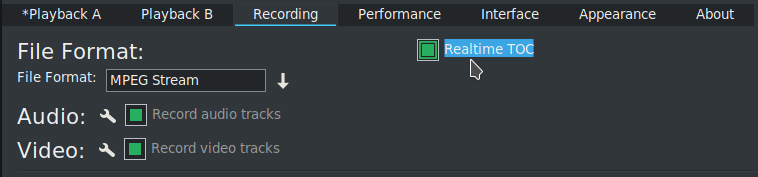
\includegraphics[width=0.8\linewidth]{realtime_toc.png}
    \caption{Realtime TOC check red button}
    \label{fig:realtime_toc}
\end{figure}

\subsection{Watching a Previously Recorded TV program}%
\label{sub:watching_recorded_tv_program}

If you have setup for DVB capture as outlined in the section above, just start here to watch a previously recorded TV program.  Use the following steps.

\begin{itemize}
    \item In the main window choose   \texttt{File $\rightarrow$ Load} files  and select the desired media file to watch.
    \item Broadcast transport streams may consist of multiple programs that all run together on one  channel (for example $9-1$, $9-2$, and $9-3$ are all on channel 9). Therefore when you play the
    recorded program back all of these programs will play simultaneously and that is a jumble. In order to select just the one you want, press Alt-1 in the main window to select \textit{Asset Program 1} (or "Alt-1...8" to select the desired asset program number) which removes all of the unrelated audio/video tracks except for the selected program. It also resets the session to match the media.
    \item Move timeline to where you would like to start watching.
    \item Be sure the Compositor window is up and you will see the pre-recorded program there.	Use either the keyboard, a remote control that has been set up, or Android device for controls.  To toggle between fullscreen or original size, press "f" in the Compositor window.
\end{itemize}

To watch on a large TV screen or monitor which you have connected, you will have to setup for \textit{Dual Screen Mode} as explained in the next section.  In addition, you can either use a Remote Control hardware device or special key setup for manipulating the playback.

\subsection{Dual Screen Mode}%
\label{sub:dual_screen_mode}

Dual screen mode is useful for displaying \CGG{} video/project on a large screen digital Television set or for watching a previously recorded broadcast TV program via \CGG{}.  The physical configuration results in one screen (an \textit{Xwindow}) on one monitor and the other screen on the other monitor or TV screen.  Before the mode is usable for \CGG{}, X has to be configured in \textit{dual screen mode} --- that is, you must first split the configuration into 2 displays to operate Dual Screen Mode.  On some systems, you may be able to get to the dual screen mode by using \textit{Xinerama} allowing for use of 2 physical displays to act as 1 virtual display.

The main menu pulldown, \texttt{Settings $\rightarrow$ Preferences $\rightarrow$ Playback A} and \texttt{B} Tabs, must be properly configured in order to take advantage of the Dual Screen Mode capability.

In the main menu Window pulldown there are \textit{Tile left} and \textit{Tile right} options for the 2 monitors.  If you have only 1 monitor, you will see no change upon activating these options.  Tiling is possible due to the existence of one long horizontal screen display buffer. Tile left takes \CGG{} and moves all of its windows to the $2^{nd}$ monitor/TV and Tile right puts it back to the $1^{st}$ monitor.  The left and right monitors are the left part or right part of a Playback A/B Xwindow host referenced in the Video Config Playback A/B for separate X screens.  Shortcuts for Tile left and Tile rights are the letters \texttt{a} and \texttt{b} on the keyboard once you have set \textit{Remote Control mode}.  Below is a summary of the configuration letters:

\begin{description}
    \item[a] select \textit{playback a} and tile windows left (all on monitor or laptop)
    \item[b] select \textit{playback b} and tile windows right (all on $2^{nd}$ monitor or TV)
    \item[c] select \textit{playback c} and tile windows left, but composer right (TV mode) This option has the effect of taking the Compositor window and moving it to the $2^{nd}$ monitor/TV without the surrounding borders interfering with the video.
\end{description}

Since Dual Screen Mode is most widely used for either a demonstration or watching TV, you will want to take advantage of Remote Control mode as described in a following section.  In the camera shots below, note the square red box that shows up in the upper left hand corner of the Viewer window (arrow pointing to it but it looks more orange than red) which denotes that the Application/Menu key was used to get into Remote Control mode.

Figure~\ref{fig:two-monitors01} shows 2 monitors (could just as well be a big-screen TV for the second monitor) with Tile left where all of the \CGG{} windows are on the left most monitor.  The big red arrow points to the little red square box indicating that Remote Control mode is in effect.

\begin{figure}[htpb]
    \centering
    \includegraphics[width=0.85\linewidth]{two-monitors01.png}
    \caption{Dual screen - initial}
    \label{fig:two-monitors01}
\end{figure}

Figure~\ref{fig:two-monitors02} shows 2 monitors with Tile right (b key) where all of the \CGG{} windows are on the right monitor.  The left monitor shows the Suse distro logo and a couple of xterm type windows.

\begin{figure}[htpb]
    \centering
    \includegraphics[width=0.85\linewidth]{two-monitors02.png}
    \caption{Dual screen - \CGG{} and desktop on different screens}
    \label{fig:two-monitors02}
\end{figure}

Figure~\ref{fig:two-monitors03} shows 2 monitors with Compositor window on the 2nd monitor which was obtained through use of the “c” keypress available when in Remote Control mode.

\begin{figure}[htpb]
    \centering
    \includegraphics[width=0.85\linewidth]{two-monitors03.png}
    \caption{Dual screen - \CGG{} compositor on own screen windowed}
    \label{fig:two-monitors03}
\end{figure}

Figure~\ref{fig:two-monitors04} shows 2 monitors with Compositor window on the 2nd monitor in Fullscreen mode so that no \CGG{} borders are visible to distract from the picture.  The big red arrow points to the little red square box indicating that Remote Control mode is in effect.

\begin{figure}[htpb]
    \centering
    \includegraphics[width=0.85\linewidth]{two-monitors04.png}
    \caption{Dual screen - \CGG{} compositor on own screen full screen}
    \label{fig:two-monitors04}
\end{figure}

\subsection{Remote Control for DVB}%
\label{sub:remote_control_dvb}

\CGG{} DVB recording/playback can now easily be done in \textit{couch potato} mode using a remote control.  This comes in handy when you want to playback on a big TV screen for multiple person viewing. You can use the Application/Menu key on the keyboard to toggle between standard \CGG{} usage or a Dispatcher methodology through use of a remote control, an Android programmed device such as a tablet, or keyboard. The Application/Menu key on most keyboards is between the Alt and Ctrl keys on the right hand side bottom and depicts a menu on it either with or without a pointer (see image below).  An ati-x10 Remote Control device (figure~\ref{fig:remote01}) is currently working with \CGG{} and other remote controls may work but have never been tried.  The red/orange box on the top left main screen of \CGG{}  indicates Dispatcher Method access is activated which allows for keyboard grab which routes all key strokes until toggled off.  Below are the currently defined operations.

\begin{figure}[htpb]
	\centering
	\includegraphics[width=0.1\linewidth]{remote01.png}
	\caption{Ati-x10 Remote}
	\label{fig:remote01}
\end{figure}

Remote Control Keys (Application/Menu key toggle for ati-x10 remote)

% Should find something so that the last column width automatically adapts to margin/font/pagesize.
\begin{tabular}{lc p{12cm}}
	\toprule
    up arrow&=&forward 1 minute\\
    
    down arrow&=&forward single frame\\
    
    left arrow&=&forward slow playback\\
    
    right arrow&=&forward normal playback\\
    
    d&=&toggle channel scan menu\\
    
    f&=&toggle full screen\\
    
    a&=&select playback a and tile windows left (all on laptop)\\
    
    b&=&select playback b and tile windows right (all on TV)\\
    
    c&=&select playback c and tile windows left, but composer right (TV mode)\\
    
    0--9&=&select timeline by 1/10s from beginning to end\\
    
    a&=&toggle audio mute\\
    
    m&=&toggle audio meters\\
    
    keypad /&=&display mpeg ts stream program data\\
    
    keypad *&=&display mpeg ts stream channel schedule date\\
    
    keypad +&=&change channel, next\\
    
    keypad -&=&change channel, prev\\
    
    keypad .&=&start channel change by numeric entry\\
    
    keypad ..&=&clear channel entry\\
    
    book key&=&toggles channel scan (always available)\\
    
    hand key&=&terminates \CGG{} (always available)\\ 
    \bottomrule 
\end{tabular}

\noindent Plus usual Transport keys:

\begin{tabular}{lcl}
	\toprule
    e&=&??\\
    
    f&=&toggle full screen\\
    
    <<&=&fast reverse\\
    
    >&=&toggles normal playback\\
    
    >>&=&fast forward\\
    
    red o&=&slow reverse\\
    
    square&=&stop\\
    
    2 lines&=&fast reverse\\
    \bottomrule   
\end{tabular}

The Application/Menu key  \quad
\includegraphics[height=\baselineskip]{alt-ctrl.png} \quad
is used to get into remote control mode, even if there is no remote control hardware device in use, allowing for use of the same defined remote control keys to work on the keyboard.  Once the Application/Menu key enables remote mode, the remote control keys don't allow the standard \CGG{} keys to work.

\subsection{Android Remote Control for DVB}%
\label{sub:android_remote_control_dvb}

\CGGI{} has Android remote interface code (figure~\ref{fig:remote02}). Any device, such as a tablet or a phone, can be used as long as it is running the Android operating system. Programming an Android Remote Control for DVB is a bit complicated at first, but becomes pretty simple after a bit.

\begin{enumerate}
    \item The Android Remote Control requires you to download and install the Android \textit{CineRmt} app package (apk). To install it simply download it (any way you can) to your phone or tablet and click it to install, if it doesn't run automatically.
    \item In \CGG{}, open \texttt{Settings $\rightarrow$ Preferences $\rightarrow$ Interface} tab, and enable \textit{Android Remote Control} in the Operation section using the checkbox. The default port $23432$ and default PIN value \textit{cinelerra} are OK.
    \item After you install the new phone/tablet app in step 1, start it up from your apps menu.
\end{enumerate}

\begin{figure}[htpb]
    \centering
    \includegraphics[width=0.9\linewidth]{remote02.png}
    \caption{Interface tab shows Android Remote Control}
    \label{fig:remote02}
\end{figure}

Before you can use it, the Android device must have the ip address of your computer entered into the configuration menu.  The PC you are running \CGG{} on and the Android device have to be on the same network.  You can tell it is in communication by tapping the \texttt{Power} (menu) button. When the remote is operated with the \textit{Power} (menu) button, there is a little orange box on the upper left corner of the display to indicate the remote state is active. If you do not see the little orange box when the menu key is tapped, the communication is broken and must be fixed before proceeding.   Follow the directions in the paragraph below.

BIG NOTICE:  the firewalls in your computer and wifi router can stop this thing dead.  Re-configuring a firewall is tricky and varies from distro to distro.  If possible, during setup it is suggested that you disable the firewall temporarily.  For those with advanced skills, use tcpdump or wireshark to look for udp messages from the IP address of the device.

SECTION NOT COMPLETE – (manualandroid)

Figure~\ref{fig:remote03} shows an Android Tablet that can be used as a Remote Control for \CGG{} Recording and Playback.

\begin{figure}[htpb]
    \centering
    \includegraphics[width=0.5\linewidth]{remote03.png}
    \caption{A Tablet with Android Remote Control}
    \label{fig:remote03}
\end{figure}

\subsection{Setup a Remote Control Device}%
\label{sub:setup_remote_control_device}

SECTION NOT DONE !! This section explains how you can take your own brand of remote control and set it up to easily work the way you want with \CGG{}.

\section{The commercial DB}%
\label{sec:commercial_db}

While watching broadcast television, it is possible to use \CGG{} to automatically mute commercials being aired during a broadcast capture.  Visual muting as well as sound muting is done!  You can NOT use ffmpeg for the format when working with the \textit{commercial DB}.  This database that was added is a \textit{novel architecture} shared memory database, a \textit{Traveling Data Base} (TDB). With TDB you have direct access to the shared database presence (instead of having to go to the server).

Basically it works as follows, but there are a few differences in just how it goes about it:

\begin{enumerate}
    \item Identify a zone in a timeline as a commercial.
    \item Characterize it concisely, in the audio and video timeline.
    \item Store the characterization in a database.
\end{enumerate}

Then, when capturing media or building a table of contents for an mpeg transport stream (broadcast capture DVB):

\begin{enumerate}
    \item Characterize each I-Frame (a few frames per sec).
    \item Search the database in real-time to identify the image.
    \item If a match is identified, automatically press the mute button.
    \item Unmute if the pattern match fails, or the commercial ends.
\end{enumerate}

It mostly works, but it takes more time to setup and maintain the database as the advertisements change frequently or vary by a small amount.  It would take a small set of personnel to keep the database current and some finessing of the code.

Currently, to activate the commercial database (db) methods you must do the following as root:

\begin{lstlisting}[style=sh]
cd <cin-path>/bin
mkdir /cinelerra              #yes, currently only in the / filesystem
./cin_db /cinelerra/media.db  #to create a new empty commercial     capture database
export BC_USE_COMMERCIALS=1   #in the command shell that is starting \CGG{}
\end{lstlisting}

This activates the gui tools and database access.  As of yet, all of the requisite permission changes
necessary to run as non-root have not been worked out (initially just easier to run as root).

When a commercial is \textit{cut}, the following occurs:

\begin{enumerate}
    \item transmits the capture timeline fragment to \texttt{/tmp}
    \item scans the snip to characterize it statistically
    \item creates a miniature b/w movie of the beginning and end
    \item stores all of this into the \texttt{media.db}
\end{enumerate}

There are 2 ways currently to identify a commercial:

\begin{enumerate}
    \item Load mpeg3 transport media, highlight select the commercial in the  timeline, and press \textit{cut commercial} on the toolbar.
    \item Use the remote control interface to indicate the boundary in/out cut points in the realtime capture timeline, and operate a cut command.    
\end{enumerate}

The cut command creates a popup to let you know that it is processing the captured data.  This can take several seconds depending on the size and media format.  The results from the scan are stored in a new record in the \texttt{media.db}.

The stats are somewhat disappointing.  Image recognition is way past zero, it is not $100$ percent. Broadcast streams have tons of minor variances which hamper digitally perfect reproduction from instance to instance of commercial presentation.  This puzzle remains to be solved.

To review media stored in the \texttt{media.db}, and delete old expired commercial data records, press (Shift-M) from the main window.  This will create a media-db window which shows the various captured samples stored there.

Currently, only a customized \textit{ati-x10} (kernel mod required) radio remote control works.  But this can quite readily be modified for other remote control models.

\section{Transfer VHS/DVD Media or Video8/Hi8 Tapes into \CGG{}}%
\label{sec:transfer_vhs_dvd_tapes_into_cinelerra}

If you want to transfer the data on a VHS tape, DVD disc, or Video8/Hi8 Tapes into \CGG{}, you
can do so by playing the media and recording while playing.  This captures the media, which you
are able to view as it plays, and writes it to a file so it can be played directly or edited.
Because there is so much variation in hardware on both the Computer side and the Media Player side,
these \textit{how to} directions are only a guideline.  You will most likely still have to do some
experimentation and testing to see what works for you.

The basic strategy consists of 3 operations:  connect the relevant outputs to representative inputs, configure the capture card to match the video, and start the Record monitor.  Each of these may have to be experimented with to get them correct for your hardware setup.

\textit{Step 1}: Connect both audio and video from your player hardware to the sound board and/or the capture card of your computer.  Sometimes the capture card handles both audio and video but oftentimes audio and video are hooked up separately.

For example in a test case using the \textit{CX23418} capture card (an older/unusual single chip MPEG-2 encoder with integrated analog video/broadcast audio decoder), one end of an S-Video cable was plugged into the back of a DVD player and the other end plugged into this computer’s Capture card; the audio was plugged into the \textit{line in} on the computer sound card.

\textit{Step 2}: Setup \CGG{} and it might be best the first time if you start with a default \texttt{.bcast5} file by using a
command line from a window of \\
\texttt{CIN\_CONFIG=\$HOME/bcast6 {cinelerra\_path}/bin/cin}

\begin{figure}[htpb]
	\centering
	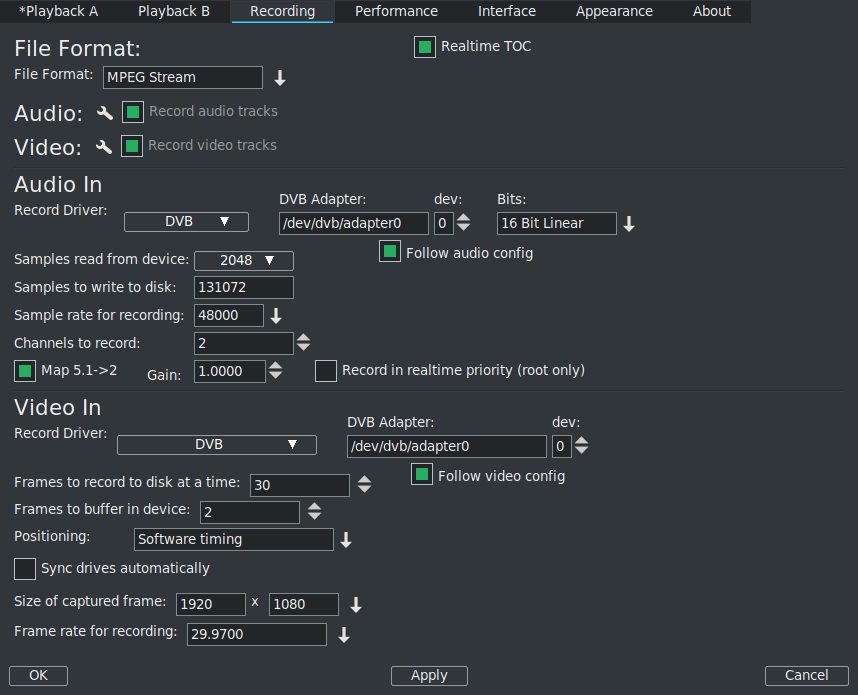
\includegraphics[width=1.0\linewidth]{recording03.png}
	\caption{Example of the Preferences menu with the Recording tab highlighted}
	\label{fig:recordingx}
\end{figure}

\begin{itemize}
    \item Choose \texttt{Settings $\rightarrow$ Preferences $\rightarrow$ Recording} tab in the Preferences menu (figure~\ref{fig:recordingx}).
    \item Choose a \textit{File Format} -- a common suggestion is \textit{ffmpeg} with a \textit{file type} of mp4.  In some cases depending on your capture card, the File Format will be set to \textit{MPEG stream} capture. Some formats support MPEG stream capture technique, otherwise the data has to be decoded first and then encoded.
    \item Check that the \textit{Audio In} section has the \textit{Record Driver} set to \textit{Alsa} with \textit{Device} set to \textit{default} as the Capture Source.  If you are using something besides Alsa, change that selection accordingly. This may not always be default and you may have to change to something else based on your specific hardware. It has to match up what you see in our Control Panel on your computer. So for example, if your device is HDMI, than the \textit{default} could be \textit{HDMI}\dots instead.
    \item In the \textit{Video In} section, change the\textit{ Record Driver} to whatever makes sense for your capture card. The test case for the CX23418 would use Video4Linux2 MPEG. A test case for an EasyCap Model \#DC60 would use Video4Linux2 JPEG.  If unknown what your card uses, you should experiment with Video4Linux2 or Screencapture as good possibilities.
    \item Also, \textit{Device path} should be verified to be correct in case you have more than 1 device. In the 2 previously mentioned devices, it should proabably be set to /dev/video0.
\end{itemize}

\textit{Step 3}: Next use the \textit{File} pulldown to choose \textit{Record} and then the Recording menu will popup (figure~\ref{fig:vhs01}).

\begin{figure}[htpb]
	\centering
	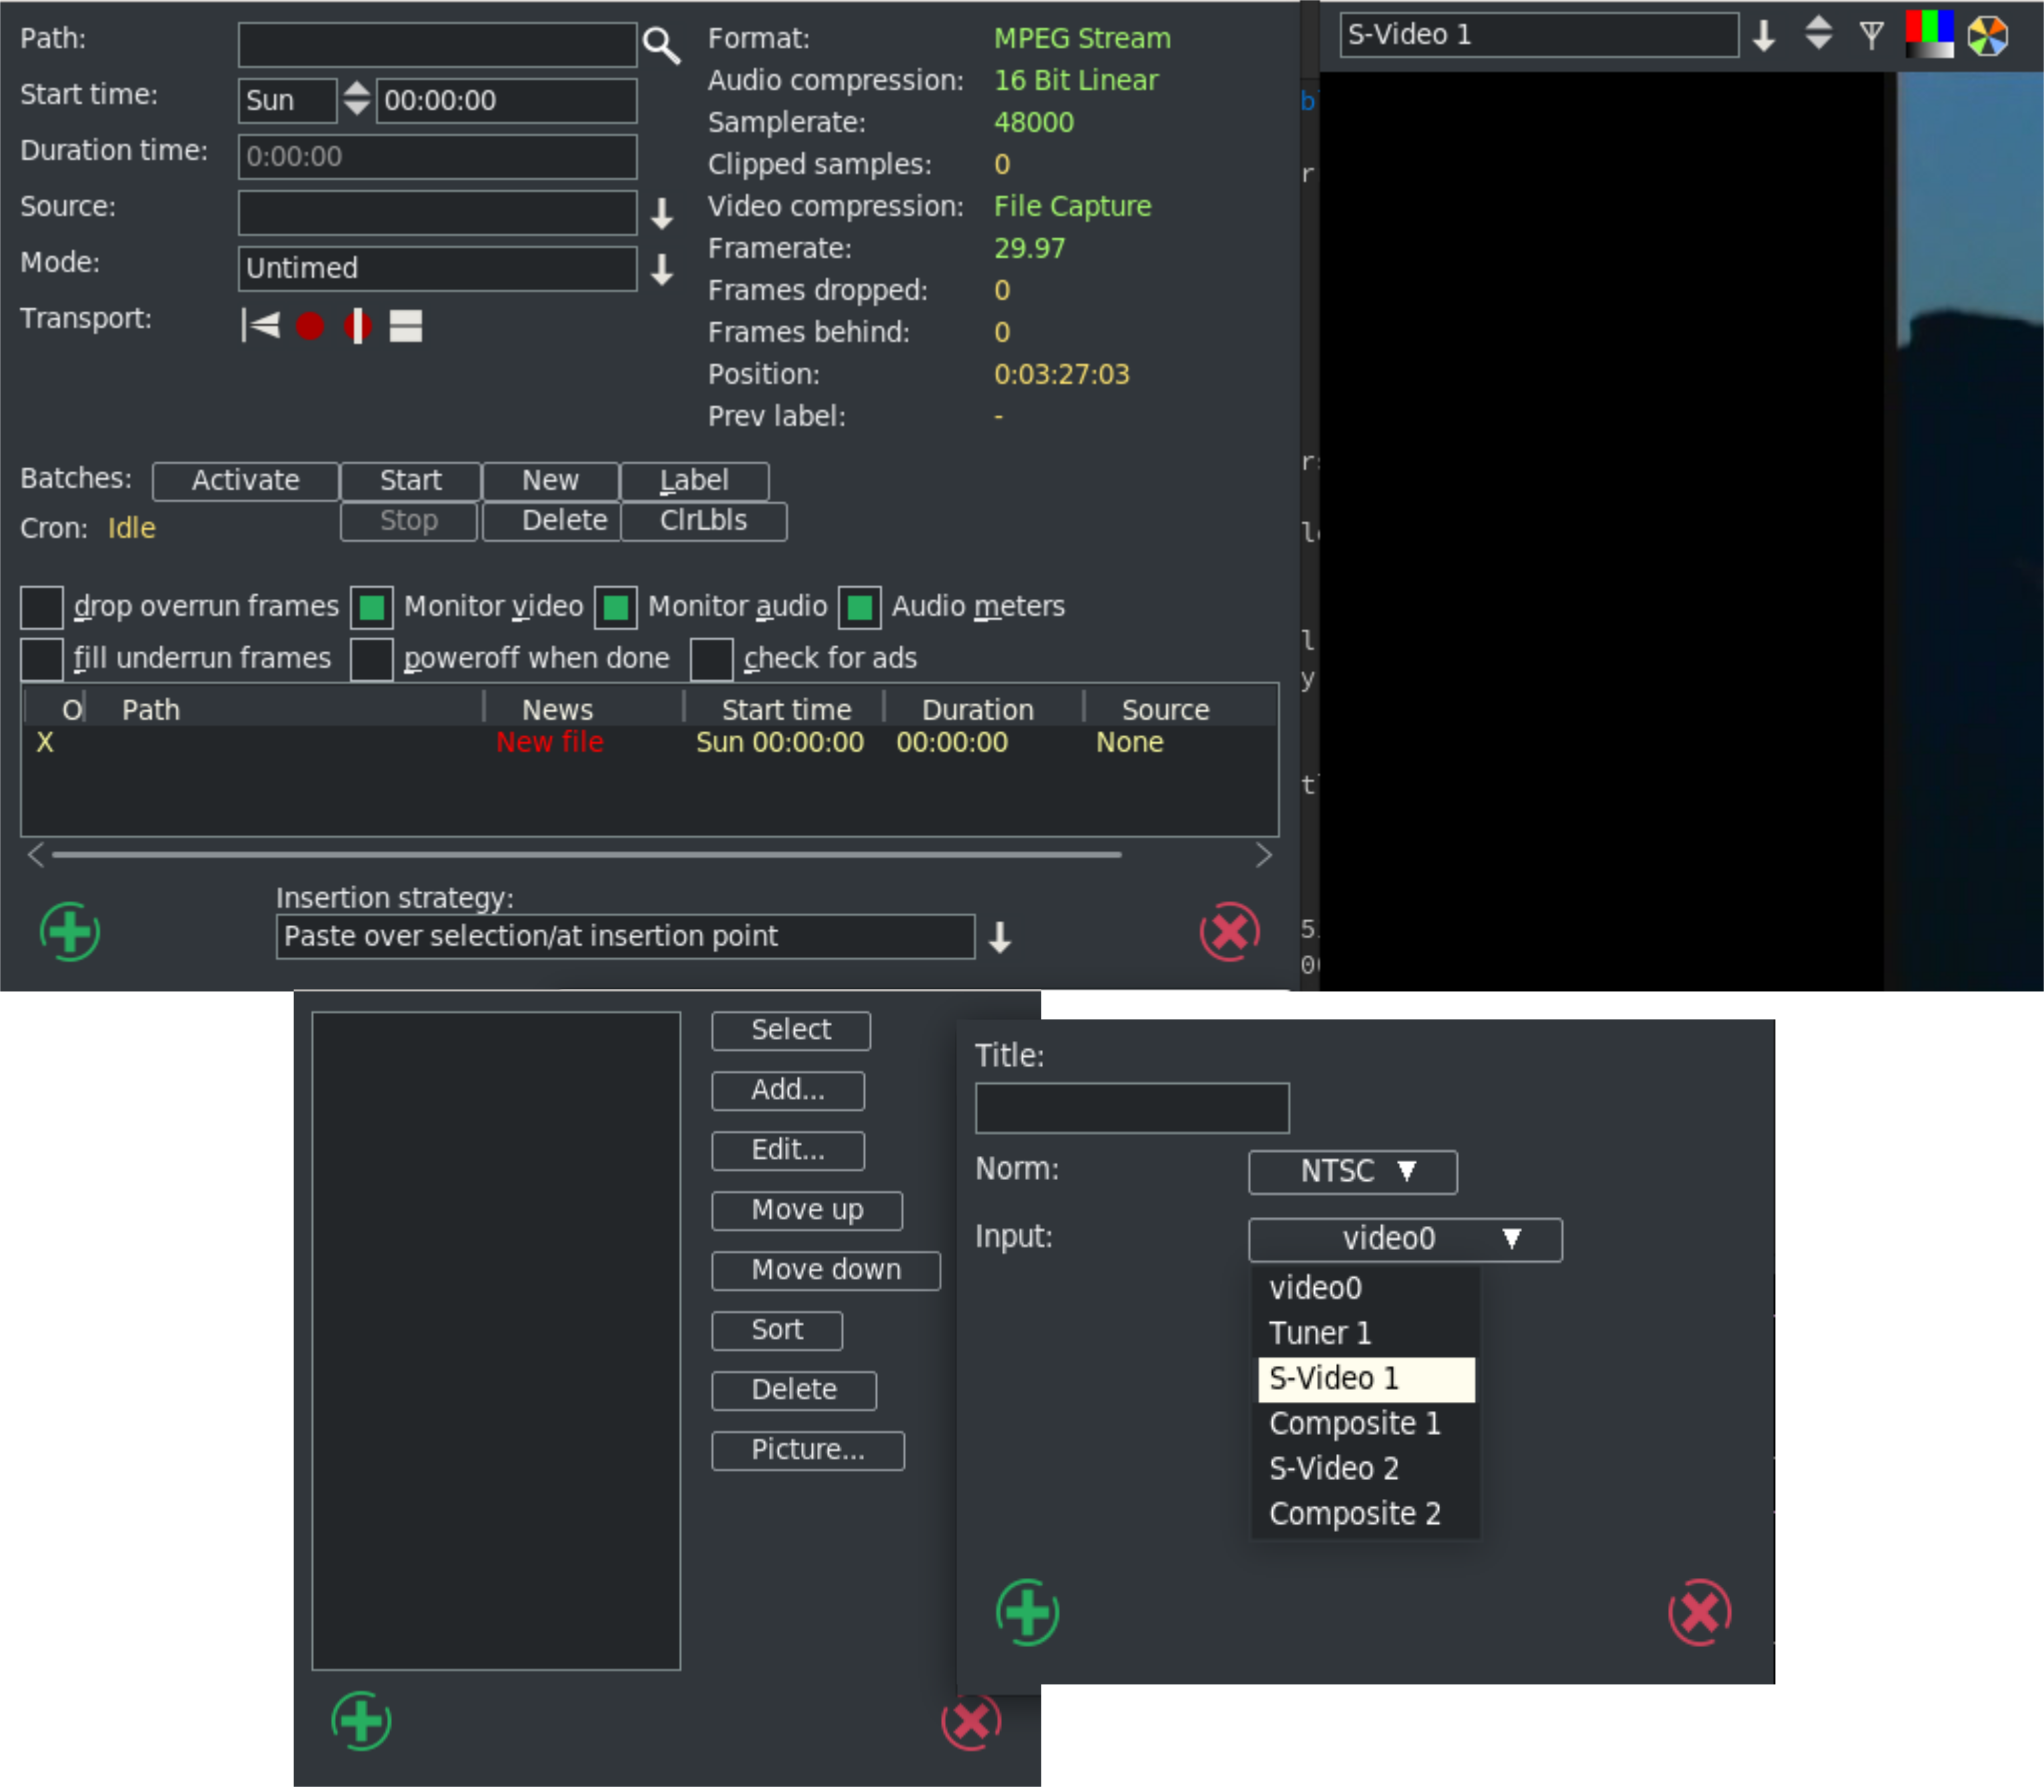
\includegraphics[width=1.0\linewidth]{vhs01.png}
	\caption{Example of the Recording, Video In, and Channels, along with the Add option, menus.}
	\label{fig:vhs01}
\end{figure}

\begin{itemize}
    \item Click on the Antenna icon ($3^{rd}$ icon from the left on the left side of the right hand screen window).
    \item In the popup \textit{Channels} menu, click on \texttt{Add} which brings up the \textit{Edit Channel} menu.
    \item Use the down arrow in the \textit{Input} box to display the available options.  In the test case, and very likely your case too, \textit{S-Video 1} should be picked.
    \item In the Recording menu, be sure to designate a complete path and filename in the \textit{Path:} textbox which will be used to record/write the playing media.  Remember you must have the media on a file in order for \CGG{} to load it on the timeline for editing purposes.
    \item Then highlight \textit{S-Video} in the \textit{Channels} Menu.  Again, the choice in the Channels Menu might not be S-Video -- choices could vary widely. Start recording in your Recording menu by clicking on the second icon from the left, next to the \textit{Transport} label (it is usually a round red colored button).
    \item Next press \textit{play} on your media hardware device.  If on the \textit{Video In} side window you see only noise, then S-Video or something else was an incorrect choice and you will have to perform some tests to find correct choices.
\end{itemize}

There are many more parameters that you may want to vary in the Recording menu or for more details on various items, please refer to the section \hyperref[sec:record_web_media_rt]{Record Web Media in real-time}. The \textit{Transport} buttons are well defined there also.

\textit{Step 4}: When the media has finished playing, use the \texttt{Stop} icon on the Recording menu – the fourth icon next to the \textit{Transport} label - to stop the recording (figure~\ref{fig:vhs02}).

\begin{figure}[htpb]
    \centering
    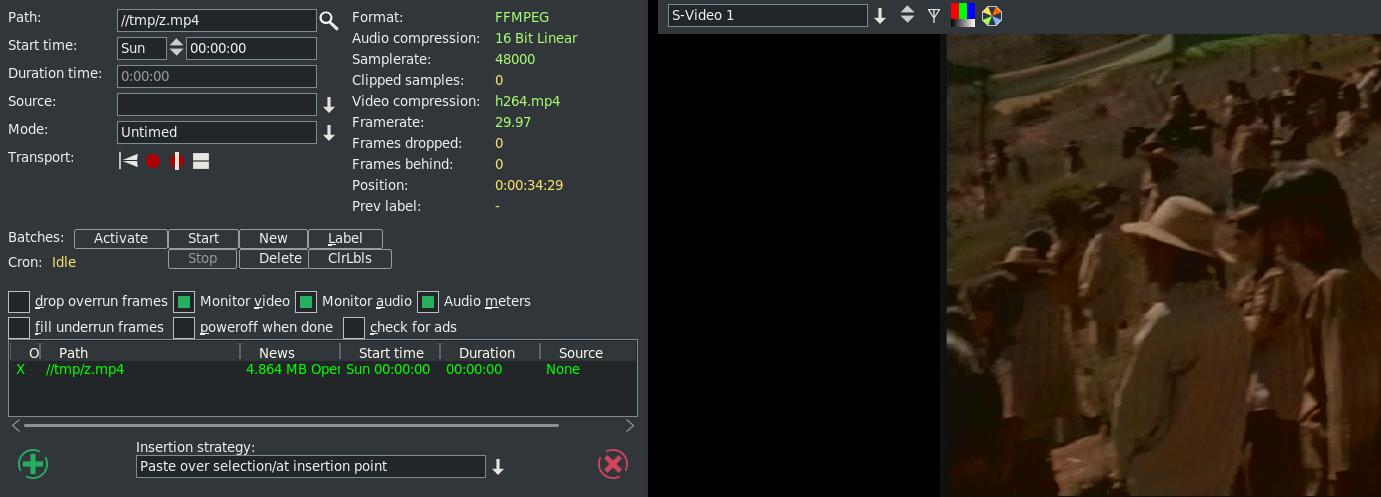
\includegraphics[width=1.0\linewidth]{vhs02.png}
    \caption{Recording menu and Video In screen while capturing media.  Note the Transport stop option.}
    \label{fig:vhs02}
\end{figure}

Now you can \textit{Load} the file that you played and recorded via the \textit{Insertion strategy} choices on the bottom of the Recording menu and edit the file as usual.  Note, that the audio and video may have started at slightly different times so you might have to initially line them up at the beginning using \texttt{nudge}.  Generally once they are correctly aligned they will stay that way.  Nudge is in the expanded patchbay. The nudge value is the amount the track is shifted left or right during playback. The track is not displayed shifted on the timeline, but it is shifted when it is played back.

\subsection{Use Case \#1 – EasyCap Model \# DC60}
\label{sub:use_case_easycap_model_dc60}

A very specific case using an Easy CAPture USB 2.0 Video Adapter with Audio, Model \#DC60 (supports
NTSC and PAL) is shown here next. The setup for this device is seen in figure~\ref{fig:recording-usb}.
A somewhat unusual choice to make note of in this image is the setting for the Video In, Record Driver
of Video4Linux2 JPEG. 

\begin{figure}[htpb]
    \centering
    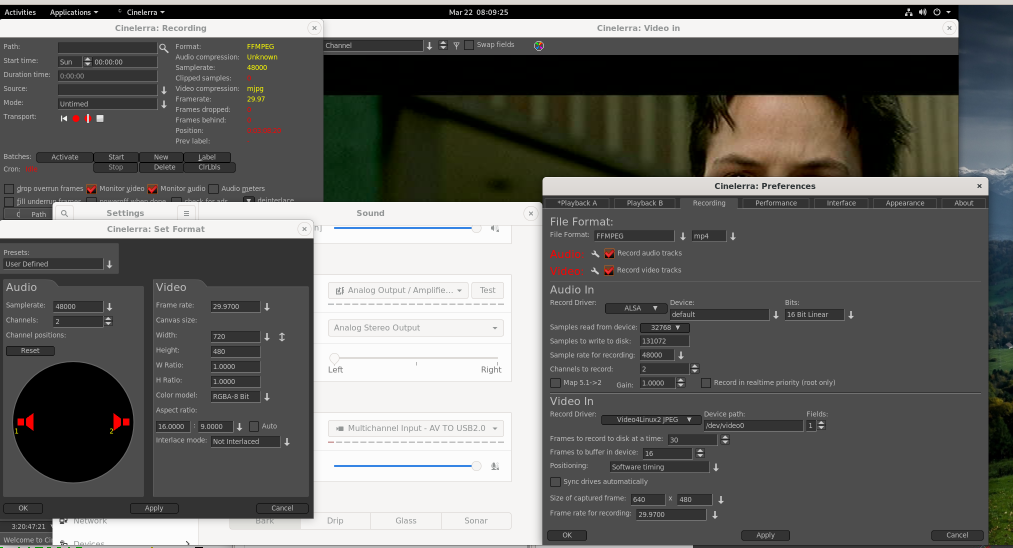
\includegraphics[width=0.9\linewidth]{recording05.png}
    \caption{Recording setup for EasyCap device}
    \label{fig:recording-usb}
\end{figure}

Output on startup window while playing:
\begin{lstlisting}[style=sh]
DeviceV4L2Base::v4l2_open pixels="MJPG"; res="480x320 640x480 720x480"
DeviceV4L2Base::v4l2_open pixels="YUYV"; res="480x320"
v4l2 s_fmt 640x480 MJPG
DeviceV4L2Base::v4l2_open VIDIOC_S_STD: Inappropriate ioctl for device
DeviceV4L2Base::v4l2_open VIDIOC_G_JPEGCOMP: Inappropriate ioctl for device
DeviceV4L2Base::v4l2_open VIDIOC_S_JPEGCOMP: Inappropriate ioctl for device
[Detaching after vfork from child process 6539]
\end{lstlisting}

\begin{lstlisting}[style=sh]
Output from "dmesg" for EasyCap - Model \# DC60:

[  748.560775] usb 3-1.2: new high-speed USB device number 8 using xhci_hcd
[  748.574296] usb 3-1.2: New USB device found, idVendor=534d, idProduct=0021, bcdDevice= 1.21
[  748.574303] usb 3-1.2: New USB device strings: Mfr=1, Product=2, SerialNumber=3
[  748.574307] usb 3-1.2: Product: AV TO USB2.0
[  748.574310] usb 3-1.2: Manufacturer: MACROSILICON
[  748.574313] usb 3-1.2: SerialNumber: 20150130
[  748.635600] hid-generic 0003:534D:0021.0008: hiddev97,hidraw0: USB HID v1.10 Device [MACROSILICON AV TO USB2.0] on usb-0000:16:00.3-1.2/input4
[  748.698491] mc: Linux media interface: v0.10
[  748.727360] videodev: Linux video capture interface: v2.00
[  748.796533] usbcore: registered new interface driver snd-usb-audio
[  748.796660] uvcvideo: Found UVC 1.00 device AV TO USB2.0 (534d:0021)
[  748.796876] uvcvideo: UVC non compliance - GET_DEF(PROBE) not supported. Enabling workaround.
[  748.797204] uvcvideo 3-1.2:1.0: Entity type for entity Processing 2 was not initialized!
[  748.797212] uvcvideo 3-1.2:1.0: Entity type for entity Camera 1 was not initialized!
[  748.797353] usbcore: registered new interface driver uvcvideo
[  748.797356] USB Video Class driver (1.1.1)
[ 3982.626522] retire_capture_urb: 7 callbacks suppressed
[ 3982.747515] usb 3-1.2: USB disconnect, device number 8
[ 4007.286371] usb 3-1.2: new high-speed USB device number 9 using xhci_hcd
[ 4007.302726] usb 3-1.2: New USB device found, idVendor=534d, idProduct=0021, bcdDevice= 1.21
[ 4007.302732] usb 3-1.2: New USB device strings: Mfr=1, Product=2, SerialNumber=3
[ 4007.302736] usb 3-1.2: Product: AV TO USB2.0
[ 4007.302740] usb 3-1.2: Manufacturer: MACROSILICON
[ 4007.302743] usb 3-1.2: SerialNumber: 20150130
[ 4007.354826] uvcvideo: Found UVC 1.00 device AV TO USB2.0 (534d:0021)
[ 4007.354939] uvcvideo: UVC non compliance - GET_DEF(PROBE) not supported. Enabling workaround.
[ 4007.355252] uvcvideo 3-1.2:1.0: Entity type for entity Processing 2 was not initialized!
[ 4007.355256] uvcvideo 3-1.2:1.0: Entity type for entity Camera 1 was not initialized!
[ 4007.420828] hid-generic 0003:534D:0021.0009: hiddev97,hidraw0: USB HID v1.10 Device [MACROSILICON AV TO USB2.0] on usb-0000:16:00.3-1.2/input4
\end{lstlisting}

\newpage

\subsection{Use Case \#2 – Hauppauge WinTV-HVR}
\label{sub:use_case_wintv}
 
In the case of the Hauppauge 9500 WinTV-HVR Hybrid TV stick, the setup is similar as in case
\#1 with the major exception being that the Video In, Record Driver should be Video4Linux2 MPEG.

\begin{figure}[htpb]
    \centering
    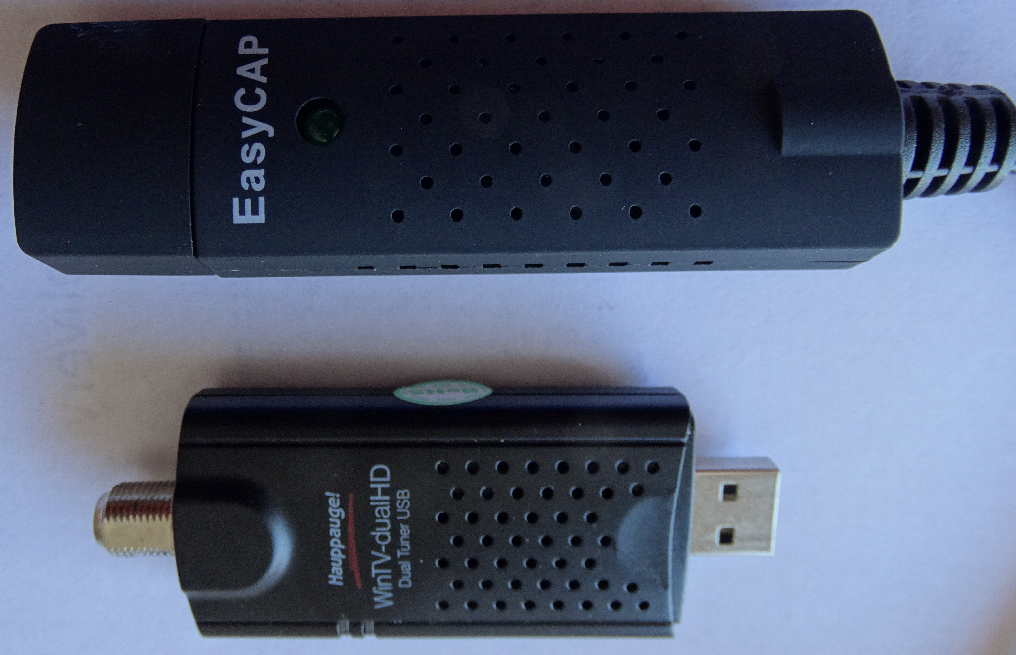
\includegraphics[width=0.6\linewidth]{recording06.png}
    \caption{Two possible capture devices using USB}
    \label{fig:recording-usb}
\end{figure}

